\documentclass[border=2pt]{standalone}
\usepackage{tikz}
\usetikzlibrary{arrows.meta,positioning,fit,backgrounds,shapes.geometric}
\usepackage{fontspec}
\setmainfont{TeXGyreTermesX}
\begin{document}
\footnotesize
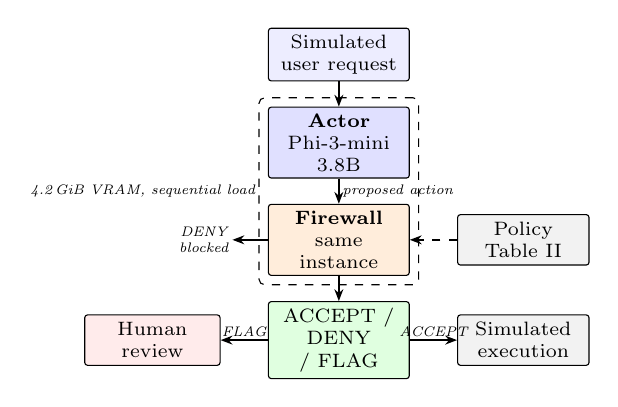
\begin{tikzpicture}[
  font=\scriptsize,
  node distance=3.2mm,
  box/.style={draw, rounded corners=1pt, align=center, inner sep=2.4pt, minimum height=6.4mm},
  arr/.style={-{Stealth[length=1.5mm]}, thick},
  lbl/.style={font=\tiny\itshape, inner sep=1pt}
]
\node[box, fill=blue!7, text width=1.62cm] (req) {Simulated\\user request};
\node[box, fill=blue!12, text width=1.62cm, below=of req] (actor) {\textbf{Actor}\\Phi-3-mini 3.8B};
\node[box, fill=orange!14, text width=1.62cm, below=of actor] (fw) {\textbf{Firewall}\\same instance};
\node[box, fill=green!12, text width=1.62cm, below=of fw] (dec) {ACCEPT /\\DENY / FLAG};
\node[box, fill=gray!10, text width=1.5cm, right=6mm of fw] (pol) {Policy\\Table II};
\node[box, fill=gray!10, text width=1.5cm, right=6mm of dec] (exe) {Simulated\\execution};
\node[box, fill=red!8, text width=1.55cm, left=6mm of dec] (human) {Human review};

\draw[arr] (req) -- (actor);
\draw[arr] (actor) -- node[lbl,right]{proposed action} (fw);
\draw[arr] (fw) -- (dec);
\draw[arr, dashed] (pol) -- (fw);
\draw[arr] (dec) -- node[lbl,above]{ACCEPT} (exe);
\draw[arr] (dec) -- node[lbl,above]{FLAG} (human);
\draw[arr] (fw.west) -- ++(-4.5mm,0) node[lbl,left,align=center]{DENY\\blocked} ;

\begin{scope}[on background layer]
\node[draw, dashed, rounded corners=2pt, fit=(actor)(fw), inner sep=3.2pt,
      label={[lbl]left:4.2\,GiB VRAM, sequential load}] (edge) {};
\end{scope}
\end{tikzpicture}
\end{document}
